\textcolor{secundario}{ESTIMACI\'ON DE LA TASA DE DESCUENTO}. La tasa de descuento generalmente aplicable a la estimaci\'on de activos intangibles puede ser calculada bajo los modelos financieros conocidos como  \gls{wacc} o \gls{wara}. Dicha tasa de descuento consiste en el rendimiento m\'inimo esperado para la organizaci\'on (\autoref{fig:op_acc} y \ref{fig:narr_val} ).

\begin{figure}[H]
\centering
\begin{minipage}{8cm}
\caption{Costo de oportunidad de los Accionistas\label{fig:op_acc}}
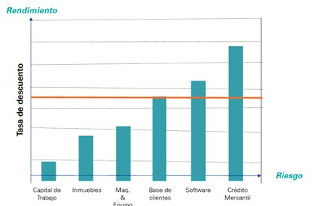
\includegraphics[height=5cm]{\rutaImagenes/costo_oportunidad_accionistas}
\footnotesize{Fuente: Valuaci\'on de Activos Intangibles. DEAL ADVISORY MEXICO. KPMG C\'ARDENAS DOSAL, S.C. KPMG ``D.R.'' \copyright 2016}
\end{minipage}
\quad
\begin{minipage}{8cm}
\caption{Fundamentos de la Narrativa Valuatoria\label{fig:narr_val}}
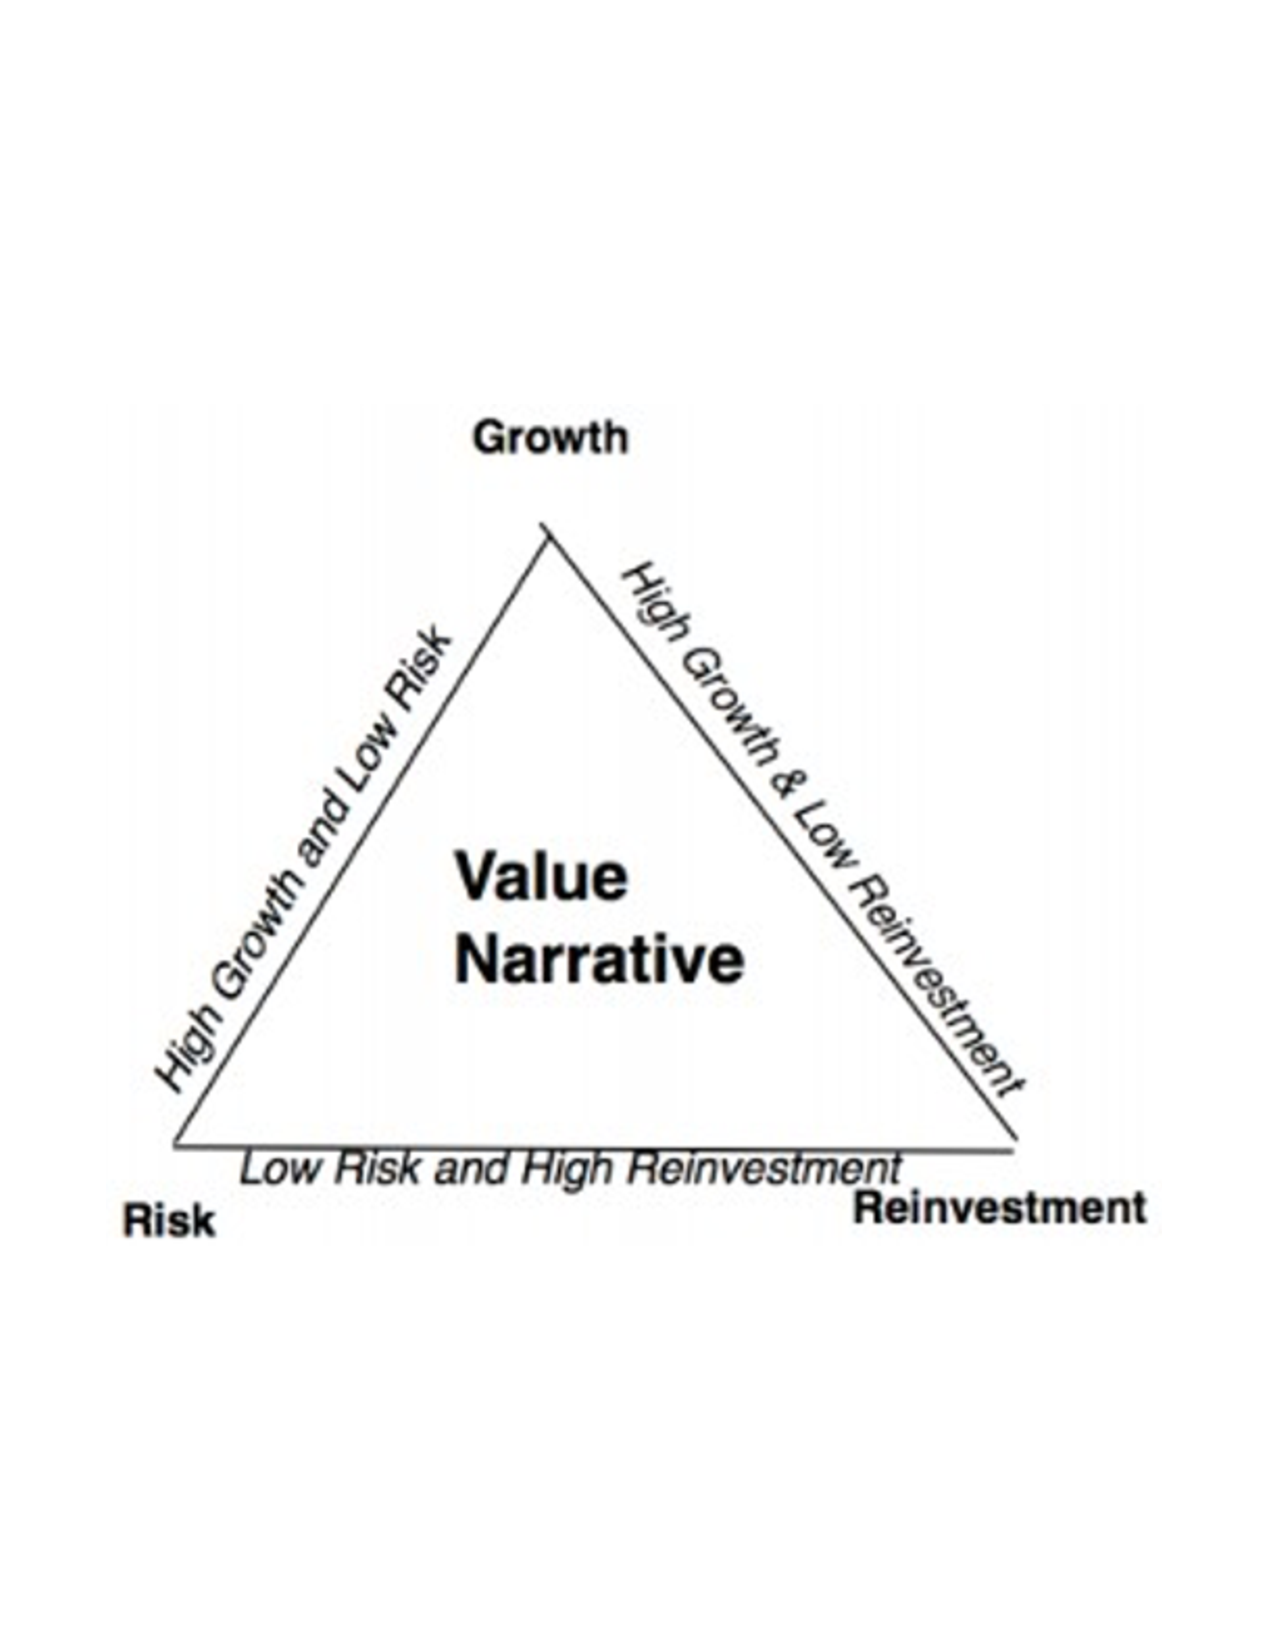
\includegraphics[height=5.5cm]{\rutaImagenes/narrativa_valuatoria}\\
\footnotesize{Fuente:Damodaran, A. ``Session 14. Narrative to numbers''. NYU/STERN.}

\end{minipage}

\end{figure}

\begin{enumerate}[i)]
\item \textcolor{secundario}{\gls{wacc} (costo promedio ponderado de capital).} El costo de capital es la compensaci\'on que los inversionistas exigen de parte de las firmas que utilizan sus fondos (costo de oportunidad).
\item \textcolor{secundario}{\gls{wara} (rendimiento del promedio ponderado de los activos).}Representa el promedio ponderado de las tasas de retorno de los Activos contributivos involucrados en la estimaci\'on del  valor razonable de un activo intangible.
\end{enumerate}

\begin{figure}[H]
\centering
\caption{Tasa de descuento WACC \& WARA.\label{fig:wacc_wara}}
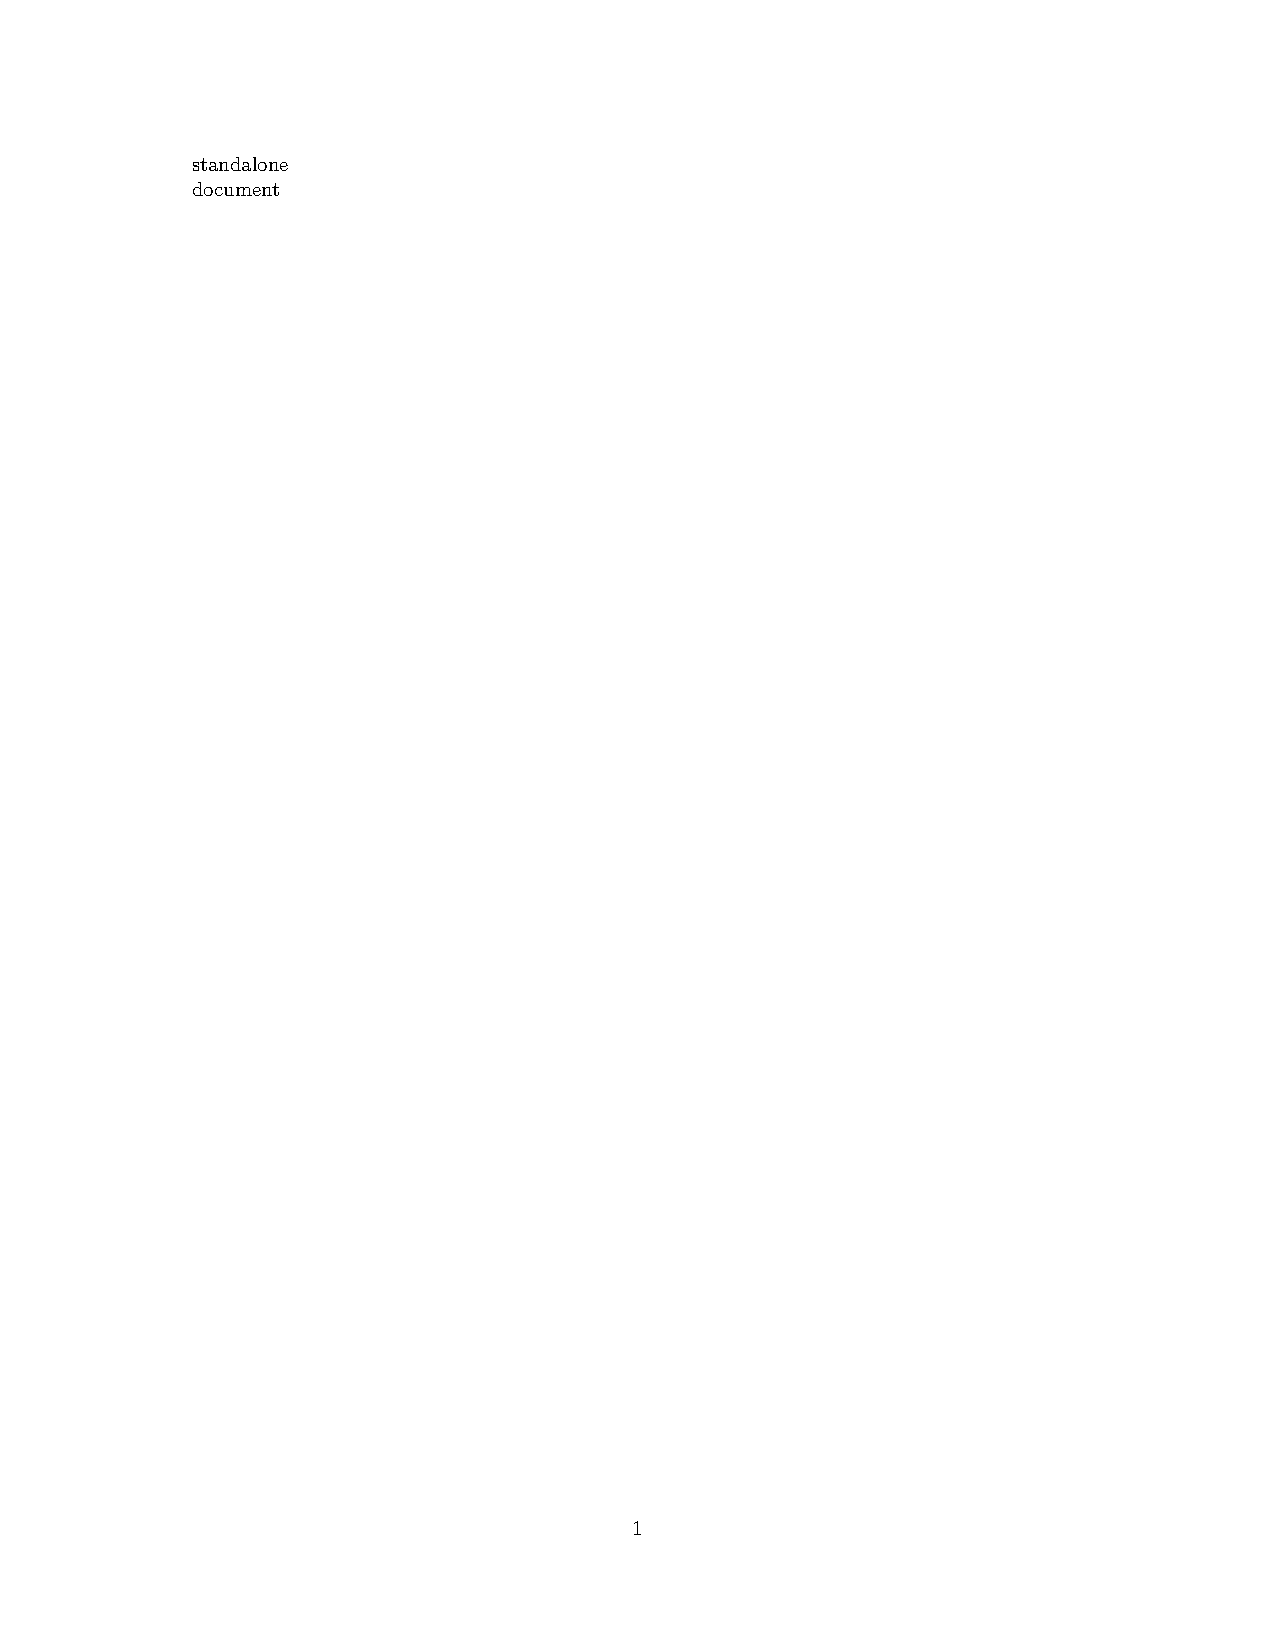
\includegraphics[width=12cm]{\rutaImagenes/wacc_wara}
\end{figure}